\documentclass{beamer}

\usepackage[francais]{babel}
\usepackage[utf8]{inputenc}
\usepackage[T1]{fontenc}

\usetheme{Warsaw}
\title{Intelligence Artificielle : promesses et réalités}
\author{Ouail Abed - Hackenolz Guillaume - Soufyani Amine}
\date{20 mars 2018}


\begin{document}

	\begin{frame}
	\titlepage
	\end{frame}
	
	\begin{frame} % 2eme transparent TDM générale
	\frametitle{Table des matieres}
	\tableofcontents[hideallsubsections] %ou [pausesections]
	\end{frame}

	
	\begin{frame}[fragile]
	\frametitle{Intelligence Artificielle : Definition}
	\begin{itemize}
		\item Intelligence Artificielle (IA)
		  est « l'ensemble de théories et de techniques mises en œuvre en vue de réaliser des machines     					  capables de simuler l'intelligence ». Elle correspond donc à un ensemble 	de concepts et de 						  technologies plus qu'à une discipline autonome constituée.
	\end{itemize}
	\end{frame}
	
	\begin{frame}[fragile]
	\frametitle{Intelligence Artificielle : Definition}
	\begin{itemize}
		\itemsep2em
		\item Souvent classée dans le groupe des sciences cognitives, elle fait appel à la neurobiologie 					computationnelle (particulièrement aux réseaux neuronaux), à la logique mathématique et à 							l'informatique. 
		
		\item Un réseau neuronal est l’association, en un graphe plus ou moins 															complexe,d’objets élémentaires, les neurones formels qui sont eux mêmes inspirées du fonctionement 		des neuronnes biologiques
	\end{itemize}
	\end{frame}
	
	
	\begin{frame}[fragile]
	\frametitle{2 Types d'IA}
	\begin{itemize}
		\itemsep0.5em
		\item IA faible  :\\
		est une intelligence artificielle non-sensible qui se concentre sur une tâche précise
		 
		 \item IA forte: \\
		est une intelligence artificielle dotée de conscience, de sensibilité et d'esprit
		\item les systèmes actuellement existants sont considérés comme des intelligences artificielles faibles
	\end{itemize}
	\end{frame}
	
	\begin{frame}[fragile]
	\frametitle{Breve Histoire de l'IA}
	\begin{itemize}
		\itemsep0.5em
		\item (1943) La naissance des ordinateurs :\\
		 Les premiers ordinateurs voient le jour. Construits avec des technologies qui précédaient les circuits 			intégrés (tubes à vide, relais électromécaniques), ils sont peu performants.
		 
		 \item (1950) Le test Turing : \\
		 Le mathématicien britannique Alan Turing publie son article "Computing Machinery and Intelligence" 			 et met au point son test à l’aveugle pour déterminer qui est l’humain ou l’ordinateur.

		 \item (1950) La première machine capable d’apprendre :\\
		 Claude Shannon développe Theseus, une souris électromécanique capable d’apprendre à trouver la 			 sortie d’un labyrinthe. Avant même l’apparition du terme "intelligence artificielle", il s’agissait de la 				 première démonstration effective d’une machine capable d’apprendre.

	\end{itemize}
	\end{frame}
	
	\begin{frame}[fragile]
	\frametitle{Breve Histoire de l'IA(suite)}
	\begin{itemize}
		\itemsep1em
		\item (1956) Le séminaire du Dartmouth College :\\
		 Les premiers ordinateurs voient le jour. Construits avec des technologies qui précédaient les circuits 			intégrés (tubes à vide, relais électromécaniques), ils sont peu performants.
		 
		 \item (1958) Le « list processing » : \\
		 John McCarthy, co-organisateur du séminaire du Dartmouth College, créé le langage informatique 				 LISP (mot forgé à partir de l’anglais "list processing") qui permet de faciliter la programmation d’IA.

		 \item (1959) Le « General Problem Solver » :\\
		 Herbert Simon et Allen Newell inventent le General Problem Solver, une stratégie de résolution de 				 problèmes largement utilisée dans le domaine de l'intelligence artificielle.

	\end{itemize}
	\end{frame}
	
	\begin{frame}[fragile]
	\frametitle{Breve Histoire de l'IA(suite)}
	\begin{itemize}
		\itemsep1em
		\item (1965) Le programme Eliza :\\
		 Eliza est un programme informatique écrit par Joseph Weizenbaum, capable de dialoguer en anglais 			en incarnant le rôle d’une psychologue.

		 \item ((1974) Le système MYCIN : \\
		 MYCIN est un système expert utilisant l’IA pour identifier des bactéries causant des infections 						sévères et recommander des antibiotiques en adaptant le dosage au poids des patients.

		 \item (1996) La victoire Deep Blue :\\
		 Le champion d’échecs Garry Kasparov est battu par le superordinateur Deep Blue d’IBM. Un 						événement qui démontre que l’IA est plus performante que l’homme dans certains domaines précis.

	\end{itemize}
	\end{frame}
	
	\begin{frame}[fragile]
	\frametitle{Breve Histoire de l'IA(suite)}
	\begin{itemize}
		\itemsep1em
		\item (2005) Le robot Stanley :\\
		 En 2005, Stanley, un robot construit à l’université Stanford, remporte le "DARPA Grand Challenge" en 		 conduisant de manière autonome pendant 131 miles sur une piste de désert sans avoir fait de 						 reconnaissance préalable
		 
		 \item (2001) Le programme Watson :\\
		 Le programme d’IA Watson d’IBM surclasse les meilleurs joueurs du jeu télévisé américain de 						 questions réponses Jeopardy !

		 \item (2017) L’AlphaGo :\\
		 En mars 2016, le programme d’IA de Google AlphaGo bat un des meilleurs joueurs mondiaux de jeu 				 de go, puis le 27 mai 2017, il bat le champion du monde Ke Jie.

	\end{itemize}
	\end{frame}
	
	\begin{frame}[fragile]
	\frametitle{Évolution de L'intelligence  Artificielle}
	
	\centerline{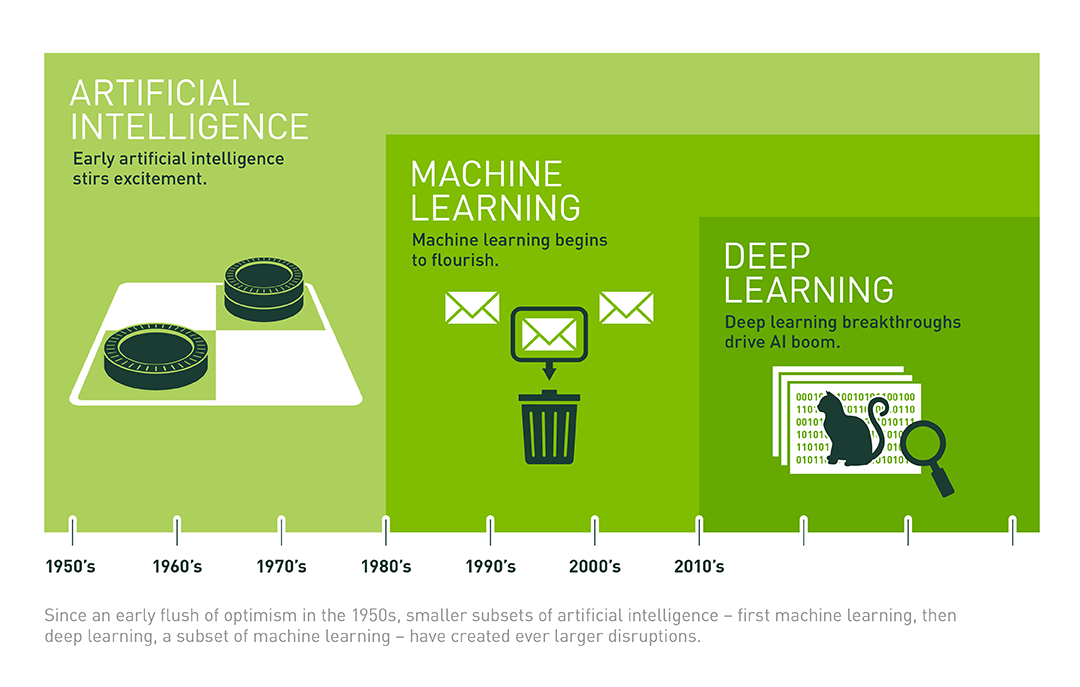
\includegraphics{evolution.png}}
	
	\end{frame}
	
	\begin{frame}[fragile]
	\frametitle{Évolution de L'intelligence  Artificielle : Machine Learning}
	\begin{itemize}
		\item Le machine learning permet à une machine d’adapter ses comportements en se fondant sur 				l’analyse des données à sa disposition. Un robot peut ainsi apprendre à marcher en commençant par 			des mouvements aléatoires, puis en sélectionnant les mouvements lui permettant d’avancer.
	\end{itemize}
	\end{frame}
	
	\begin{frame}[fragile]
	\frametitle{Évolution de L'intelligence  Artificielle : Deep Learning}
	\begin{itemize}
		\itemsep1em
		\item Le deep learning est la branche du machine learning qui utilise comme modèles mathématiques 			les réseaux de neurones formels, eux-mêmes construits sur la représentation mathématique et 					informatique d’un neurone biologique, née en 1943.
		\item  Le Deep Learning est utilisé dans la voiture autonome  de Google : le réseau de  neurones 					classifie tout l’environnement pour éviter les obstacles ou s’arrêter au bon moment 
	\end{itemize}
	\end{frame}
	
	\begin{frame}[fragile]
	\frametitle{Évolution de L'intelligence  Artificielle}
	
	\centerline{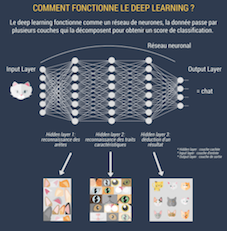
\includegraphics{deeplearning.png}}%changer pour image de meilleure qualitée
	
	\end{frame}
	
	\begin{frame}[fragile]
		\frametitle{Évolution de L'intelligence  Artificielle (fin)}
		\begin{itemize}
		\item Ces deux branches de l'intelligence artificielle ont causées de grandes améliorations de 						algorithmes, mais malgres cela l'IA d'aujourd'hui est est toujours qualifiée de « faible », en opposition 			à l’IA « forte » et consciente d’elle-même que prédisent les transhumanistes.

	\end{itemize}
	\end{frame}
	
	\begin{frame}[fragile]
		\frametitle{Le Test De Turing : Definition}
		\begin{itemize}
		 \item Le test de Turing est une proposition de test d’intelligence artificielle fondée sur la faculté d'une machine à imiter la conversation humaine. Décrit par Alan Turing en 1950 dans sa publication Computing machinery and intelligence, ce test consiste à mettre un humain en confrontation verbale à l’aveugle avec un ordinateur et un autre humain \\
		 Si la personne qui engage les conversations n’est pas capable de dire lequel de ses interlocuteurs est un ordinateur, on peut considérer que le logiciel de l’ordinateur a passé avec succès le test. Cela sous-entend que l’ordinateur et l’humain essaieront d’avoir une apparence sémantique humaine.
		
		\end{itemize}
		\end{frame}
		
	\begin{frame}[fragile]
		\frametitle{Schema Test De Turing}
		
		\centerline{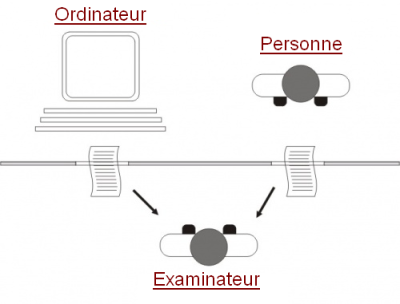
\includegraphics[scale = 0.7]{test-de-turing.png}}
	%	\centerline{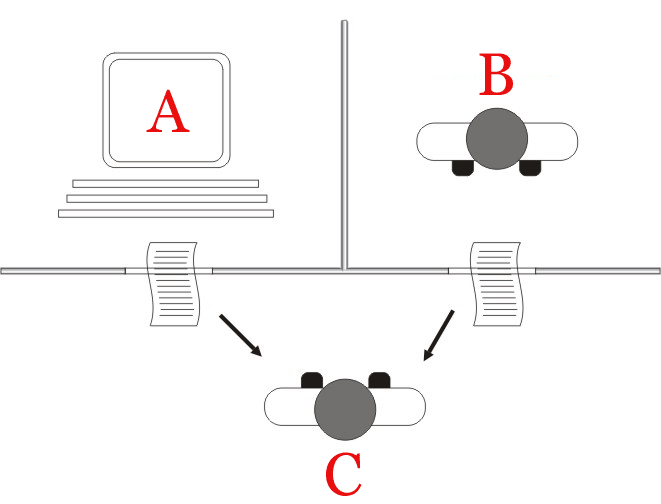
\includegraphics[0.5]{TuringTest.png}}
	
	\end{frame}
	
	\begin{frame}
		\frametitle{Outils}
		\begin{itemize}
			\item Au cours d'une soixantaine d'années de recherche, l'IA a développé plusieurs outils pour résoudre les problèmes les plus difficiles en informatique.
			\item Recherche et Optimisation
			\item Logique
			\item Classificateurs et méthodes d'apprentissage statistique
			\item Réseaux de neurones artificiels
		\end{itemize}
	\end{frame}
	
	\begin{frame}[fragile]
		\frametitle{Recherche et Optimisation}
		\begin{itemize}
		    \item Selon le scénario, il peut y avoir une ou plusieurs solutions à un problème donné, car il peut y avoir plusieurs façons de résoudre ce problème. 
		    \item Disons qu'on doit faire quelque chose comme une multiplication mathématique. Clairement, il y a une solution correcte, mais de nombreux algorithmes pour multiplier. Maintenant, prenant un problème plus compliqué, comme jouer à un jeu, Dans la plupart des cas, à un moment donné, on a plusieurs mouvements qu'on peut faire, et on choisit celui qui nous donne le meilleur résultat possible. Les agents rationnels de l'intelligence artificielle abordent les problèmes de la même manière.
		\end{itemize}
	\end{frame}
	
	
	\begin{frame}[fragile]
		\frametitle{Logique}
		\begin{itemize}
		    \item La logique a joué un rôle important dans le développement de l'Intelligence Artificielle (IA). À son tour, penser à des applications dans l'IA a conduit au développement de nombreux systèmes logiques nouveaux et intéressants.
		    \item Par exemple, l'algorithme satplan utilise la logique pour la planification. Il convertit l'instance de problème de planification en une instance du problème de satisfissabilité booléenne, qui est ensuite résolue à l'aide d'une méthode permettant d'établir la satisfiabilité.
		\end{itemize} %not finished yet
	\end{frame}
	
	
	\begin{frame}[fragile]
		\frametitle{Classificateurs et méthodes d'apprentissage statistique}
		\begin{itemize}
			\item la classification constitue une partie centrale de nombreux systèmes d'IA. 
             \item Les classificateurs sont des fonctions qui utilisent la correspondance de modèle pour déterminer la correspondance la plus proche. Un classificateur peut être formé de différentes manières; il existe de nombreuses approches statistiques et d'apprentissage automatique. L'arbre de décision est peut-être l'algorithme d'apprentissage automatique le plus utilisé.
		\end{itemize} %not finished yet
	\end{frame}
	
	
	\begin{frame}[fragile]
		\frametitle{Réseaux de neurones artificiels}
		\begin{itemize}
		    \item  c'est un système dont la conception est à l'origine schématiquement inspirée du fonctionnement des neurones biologiques, et qui par la suite s'est rapproché des méthodes statistiques.
		    \item Les réseaux de neurones sont généralement optimisés par des méthodes d’apprentissage de type probabiliste, en particulier bayésien.dans la famille des méthodes de l’intelligence artificielle auxquelles ils fournissent un mécanisme perceptif indépendant des idées propres de l'implémenteur, et fournissant des informations d'entrée au raisonnement logique formel.
		\end{itemize}  %not finished yet 
		
	\end{frame}


	
 	\begin{frame}
 	   \frametitle{Domaines D'applications}
 	   \begin{itemize}
 	    \item Finance et L'economie
 	    \item La Sante
 	    \item L'Automobile
 	    \item Jeux Video
 	   \end{itemize}
 	\end{frame}
 	
 	
 	\begin{frame}
 	   \frametitle{Finance et L'economie}
 	        \begin{itemize}
 	            \item L'utilisation de machines IA sur le marché dans des applications telles que le commerce en ligne et la prise de décision a modifié les principales théories économiques. Par exemple, les plates-formes d'achat et de vente basées sur l'IA ont modifié la loi de l'offre et de la demande. les courbes de demande et d'offre et donc les prix individualisés
 	            
 	            \item Les banques utilisent aujourd'hui des systèmes d'intelligence artificielle pour organiser les opérations, tenir la comptabilité, investir dans les stocks et gérer les propriétés.
 	           
 	            \item L'IA a également réduit la fraude et les délits financiers en surveillant les comportements des utilisateurs en cas de changements ou d'anomalies anormaux.
 	        \end{itemize}
 	\end{frame}
 	
 	
 	\begin{frame}
 	   \frametitle{La Sante}
 	   \begin{itemize}
 	       \item des algorithmes et des logiciels sont utilisés pour approcher la cognition humaine dans l'analyse de données médicales complexes. Les programmes d'IA ont été développés et appliqués à des pratiques telles que les processus de diagnostic, le développement de protocoles de traitement, le développement de médicaments, la médecine personnalisée et la surveillance des patients, soin, entre autres.
 	       
 	       \item Par exemple ll y a une grande quantité de recherche et de médicaments développés en rapport avec le cancer. Dans le détail, il y a plus de 800 médicaments et vaccins pour traiter le cancer,et pour cela  Microsoft travaille sur un projet de développement d'une machine appelée "Hanover".
 	       
 	   \end{itemize}
 	\end{frame}
 	
 	
 		\begin{frame}
 	   \frametitle{La Sante}
 	   \begin{itemize}
 	   \item Il y a eu une étude récente réalisée par des chirurgiens du Children's National Medical Center de Washington qui a démontré avec succès la chirurgie avec un robot autonome. L'équipe a supervisé le robot pendant qu'il pratiquait une chirurgie des tissus mous, en cousant ensemble l'intestin d'un cochon pendant une chirurgie ouverte, et en le faisant mieux qu'un chirurgien humain.
 	   \end{itemize}
 	 \end{frame}
 	
 	
 	\begin{frame}
 	   \frametitle{L'Automobile}
 	   \begin{itemize}
 	       \item Les progrès de l'IA ont contribué à la croissance de l'industrie automobile grâce à la création et à l'évolution de véhicules autonomes. En 2016, plus de 30 entreprises utilisent l'IA pour la création de voitures sans conducteur. Quelques entreprises impliquées dans l'IA incluent Tesla et Google.
 	       
 	       \item De nombreux composants contribuent au fonctionnement des voitures autonomes. Ces véhicules intègrent des systèmes tels que le freinage, le changement de voie, la prévention des collisions, la navigation et la cartographie. Ensemble, ces systèmes, ainsi que les ordinateurs haute performance, sont intégrés dans un véhicule complexe.
 	   \end{itemize}
 	\end{frame}
 	
 	
 	\begin{frame}
 	   \frametitle{Jeux Video}
 	   \begin{itemize}
 	       \item Dans les jeux vidéo, l'intelligence artificielle est couramment utilisée pour générer un comportement dynamique dynamique dans les personnages non-joueurs (PNJ). De plus, des techniques d'IA bien comprises sont couramment utilisées pour le pathfinding.
 	   \end{itemize}
 	\end{frame}


\end{document}